\section{Funkcije pogreške}
Iako smo pokazali da su generativne suparničke mreže asimptotski konzistentne ako kao funkciju cilja koristimo izraz \ref{orig_loss}, predstavljen u originalnom radu, budući da u praksi koristimo modele za koje pretpostavke na kojima se asimptotska konzistentnost temelji ne vrijede, istraživači su predlagali različite alternative da bi pospješili rezultate. U osnovi, predložene funkcije su formulacije različito definiranih udaljenosti između distribucija koje pokušavamo minimizirati. Osim originalne funkcije cilja i njezine modifikacije koja teži izbjeći zasićenje rano u učenju, postoje još dvije funkcije gubitka koje se češće koriste: Wassersteinov gubitak i gubitak najmanjih kvadrata. O njima će više riječi biti u nastavku poglavlja.

\subsection{Wassersteinov gubitak}
Wassersteinov gubitak \citep{arjovsky2017wasserstein} temelji se na minimizaciji udaljenosti pomicanja zemlje \engl{Earth Mover's Distance, EM}, još nazvane i Wasserstein-1 udaljenosti. EM udaljenost između distribucija $P$ i $Q$ definirana je kao:
\begin{equation}
\label{em_distance}
\operatorname*{EM}(P, Q) = \inf_{\gamma \in \Pi(P, Q)} \mathbb{E}_{(x, y) \sim \gamma} \left[ \|x - y\|\right]
\end{equation}
gdje $\Pi(P, Q)$ označava skup svih zajedničkih vjerojatnosti $\gamma(x, y)$ čije su marginalne razdiobe $P$ i $Q$, odnosno $P = \int \gamma(x, y)dy$ i $Q = \int \gamma(x, y)dx$. Oznaka $\inf$ označava infimum skupa - najveću vrijednost koja je manja od svih elemenata skupa. Intuitivno - i po ovoj je analogiji udaljenost pomicanja zemlje i dobila ime - zamislimo distribuciju $P$ kao hrpu zemlje, a $Q$ kao drugačiji način raspoređivanja zemlje na hrpu. EM udaljenost mjeri najmanju količinu rada potrebnu da bi se zemlja premjestila tako da iz hrpe $P$ dobijemo hrpu $Q$ (slika \ref{emd}).

\begin{figure}[h]
\centering
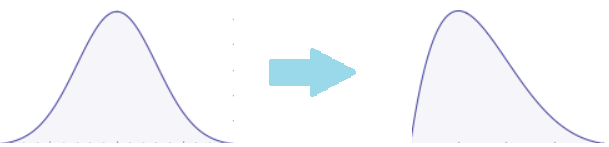
\includegraphics[width=0.7\textwidth]{images/emd.png}
\caption{Vizualizacija ideje udaljenosti pomicanja zemlje}
\label{emd}
\end{figure}

Problem u izrazu \ref{em_distance} jest što je vremenski veoma skupo odrediti traženi infinum skupa. Autori se zato koriste Kantorovič -- Rubinsteinovom dualnosti gdje se Wassersteinova udaljenost reformulira na sljedeći način:
\begin{equation}
\label{kr_dual}
W(P, Q) = \sup_{\|f\|_L \leq 1} \mathbb{E}_{x \sim P} \left[f(x)\right] - \mathbb{E}_{x \sim Q}\left[f(x)\right]
\end{equation}
Ovdje $\sup$ označava supremum skupa - najmanju vrijednost veću od svih elemenata skupa. U ovom slučaju, tražimo supremum po svim funkcijama $f : \mathcal{X} \rightarrow \mathbb{R}$ koje zadovoljavaju 1-Lipschitzovu neprekidnost. Ovo je nešto stroži zahtjev od same neprekidnosti. Općenito, $K$-Lipschitzova neprekidnost \citep{lip_cont} funkcije znači da, odaberemo li bilo koje dvije točke na grafu, apsolutna vrijednost nagiba njihove spojnice bit će manja od $K$. Vizualno, možemo provjeriti je li to svojstvo zadovoljeno u nekoj točki funkcije ako povučemo pravce nagiba $K$ kroz danu točku (slika \ref{lip_cont}).
 
\begin{figure}[h]
\centering
		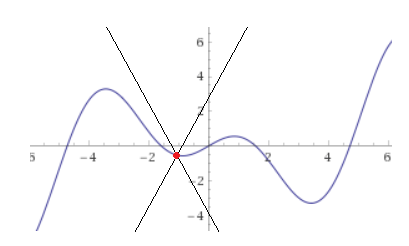
\includegraphics[width=0.7\textwidth]{images/lip_cont.png}
\caption{Vizualno ispitivanje $K$-Lipschitzove neprekidnosti. Ako kroz danu točku povučemo pravce čija je apsolutna vrijednost nagiba $K$, ravninu dijelimo na 4 dijela. Ako se ostatak grafa tada ne nalazi u gornjem i donjem području ravnine opisanom pravcima, tada je uvjet neprekidnosti zadovoljen.}
\label{lip_cont}
\end{figure}

Nadalje, može se pokazati da, ako u izrazu \ref{kr_dual} odaberemo $K > 1$, rezultat će biti $K \cdot W(P, Q)$. Ako imamo klasu funkcija parametriziranu parametrima $\vec{\theta}$ (ovo je u našem slučaju diskriminator), gdje sve zadovoljavaju Lipschitzovu neprekidnost za neki $K$, i optimum se postiže za neke $\vec{\theta}^*$, dobivamo vrijednost $K \cdot W(P, Q)$. Dakle, izraz \ref{kr_dual}, u kontekstu generativnih suparničkih mreža, možemo formulirati u sljedeći optimizacijski problem:
\begin{equation}
\max \mathbb{E}_{\vec{x} \sim p_{\mathcal{D}}} \left[D(\vec{x})\right] - \mathbb{E}_{\vec{z} \sim p_{\vec{z}}}\left[D(G(\vec{z}))\right]
\end{equation}
Iz ovog izraza, lako je odrediti gradijent generatora i diskriminatora koji su nam potrebni da bismo ih istrenirali. Jedini zahtjev je da diskriminator zadovoljava 1-Lipschitzovu neprekidnost. U tu svrhu, autori predlažu ograničavanje težina na neki mali interval, npr. [-0.1, 0.1]. Iako su postigli zadovoljavajuće rezultate, napominju da je pristup vrlo jednostavan i ostavlja prostor za druge metode osiguravanja traženog ograničenja.

Koja bi bila prednost ove funkcije gubitka u odnosu na originalno predloženu? Autori su pokazali da obje ranije predložene varijante imaju problem s iščezavajućim gradijentima, dok njihova funkcija gubitka rezultira konzistentnim gradijentima tijekom treniranja. Još jedna važna razlika u odnosu na originalan gubitak jest da izlaz diskriminatora u ovom slučaju nije vjerojatnost te zato nije ni ograničen.

\subsection{Gubitak najmanjih kvadrata}
Gubitak najmanjih kvadrata \citep{mao2016squares} razvijen je s istom motivacijom kao i Wassersteinov gubitak: da bi se izbjegao problem iščezavajućih gradijenata. Budući da originalna formulacija funkcije gubitka koristi sigmoidalnu funkciju pri klasifikaciji, gradijent za uzorke koji uspješno zavaraju diskriminator (tj. koji se nalaze s dobre strane decizijske granice), a koji su još uvijek prilično različiti od stvarnih primjera, jest nizak (slika \ref{ls_sigm}). 

\begin{figure}[h]
\centering
		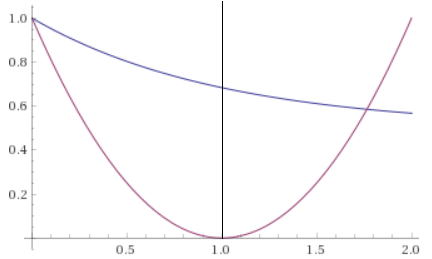
\includegraphics[width=0.7\textwidth]{images/ls_sigm.png}
\caption{Vizualna usporedba gubitka sigmoide (plavo) i kvadratnog gubitka (ljubičasto). Crno je naznačena granica između ispravno i neispravno klasificiranih primjera.}
\label{ls_sigm}
\end{figure}

Zato autori predlažu pogrešku najmanjih kvadrata za funkciju gubitka. Recimo da smo stvarne primjere označili s $a$, lažne s $b$, dok smo s $c$ označili vrijednost kojoj generator teži da bude izlaz diskriminatora. Tada bi optimizacijski problemi za generator $G$ i diskriminator $D$ glasili:
\begin{equation}
\label{ls_d}
\min_D V(D) = \frac{1}{2}\mathbb{E}_{\vec{x} \sim p_{\mathcal{D}}}\left[(D(\vec{x}) - b)^2\right] + \frac{1}{2}\mathbb{E}_{\vec{z} \sim p_{\vec{z}}}\left[(D(G(\vec{z})) - a)^2\right]
\end{equation}
\begin{equation}
\label{ls_g}
\min_G V(G) = \frac{1}{2}\mathbb{E}_{\vec{x} \sim p_{\mathcal{D}}}\left[(D(\vec{x}) - c)^2\right] + \frac{1}{2}\mathbb{E}_{\vec{z} \sim p_{\vec{z}}}\left[(D(G(\vec{z})) - c)^2\right]
\end{equation}
Radi simetričnosti, uključili smo izraz koji koristi samo izlaz diskriminatora u izraz \ref{ls_g}. Pri optimizaciji ova matematička akrobacija ne utječe na rezultat jer se spomenuti izraz gubi prilikom računanja gradijenta, ali olakšava dokazati određene povoljne karakteristike ovog gubitka. Naime, pomoću izraza \ref{ls_d} i \ref{ls_g} možemo pokazati da minimizacija gubitka najmanjih kvadrata vodi prema minimizaciji Pearsonove $\chi^2$ divergencije, još jedne mjere za udaljenost između dvije distribucije. Pearsonova $\chi^2$ divergencija između distribucija $P$ i $Q$ definirana je kao $D_{\chi^2}(P\|Q) = \int_{\mathcal{X}} (\frac{(P(x) - Q(x))^2}{Q(x)}dx$

Iz izraza \ref{ls_d} možemo pronaći optimalni diskriminator $D^*$ ako fiksiramo generator $G$. Uz fiksirani generator, \ref{ls_g} postaje
\begin{align}
V(D) &= \frac{1}{2}\mathbb{E}_{\vec{x} \sim p_{\mathcal{D}}}\left[(D(\vec{x}) - b)^2\right] + \frac{1}{2}\mathbb{E}_{\vec{x} \sim p_{model}}\left[(D(\vec{x}) - a)^2\right] \\
	&= \frac{1}{2} \int_{\mathcal{X}} \left[ p_{\mathcal{D}}(\vec{x})(D(\vec{x}) - b)^2 + p_{model}(\vec{x})(D(\vec{x}) - a)^2\right]dx
\end{align}
Podintegralna funkcija je oblika $F(y) = \frac{1}{2} \left[ e(y - b)^2 + f(y - a)^2\right]$. Lako je pokazati da je minimum ove funkcije u točki $y^* = \frac{b\cdot e + a \cdot f}{e + f}$. Obavimo li potrebne supstitucije, dobivamo:
\begin{equation}
D^*(\vec{x}) = \frac{bp_{\mathcal{D}}(\vec{x}) + ap_{model}(\vec{x})}{p_{\mathcal{D}}(\vec{x}) + p_{model}(\vec{x})}
\end{equation}
Uvrstimo li dobiveni izraz u \ref{ls_g}, dobivamo:
\begin{align*}
2V(G) &= \mathbb{E}_{\vec{x} \sim p_{\mathcal{D}}}\left[(D^*(\vec{x}) - c)^2\right] + \mathbb{E}_{\vec{x} \sim p_{model}}\left[(D^*(\vec{x}) - c)^2\right] \\
	&= \int_{\mathcal{X}} \left(p_{\mathcal{D}}(\vec{x}) + p_{model}(\vec{x})\right)\left(D^*(\vec{x}) - c\right)^2dx \\
	&= \int_{\mathcal{X}} \left(p_{\mathcal{D}}(\vec{x}) + p_{model}(\vec{x})\right) \left(\frac{(b - c)p_{\mathcal{D}}(\vec{x}) + (a - c)p_{model}(\vec{x})}{p_{\mathcal{D}}(\vec{x}) + p_{model}(\vec{x})}\right)^2 dx
\end{align*}
Radi jednostavnosti, postavimo $b - c = 1$ i $a - c = -1$. Tada imamo:
\begin{align*}
2V(G) &= \int_{\mathcal{X}} \frac{\left(p_{\mathcal{D}}(\vec{x}) - p_{model}(\vec{x})\right)^2}{p_{\mathcal{D}}(\vec{x}) + p_{model}(\vec{x})} dx
	&= \int_{\mathcal{X}} \frac{\left(p_{\mathcal{D}}(\vec{x}) + p_{model}(\vec{x}) - 2p_{model}(\vec{x})\right)^2}{p_{\mathcal{D}}(\vec{x}) + p_{model}(\vec{x})} dx \\
	&= D_{\chi^2}(2p_{model}\|p_{model} + p_{\mathcal{D}})
\end{align*}
Ovime smo dokazali da pronalazak optimalnih težina pomoću ovog gubitka minimizira Pearsonovu $\chi^2$ divergenciju između $2p_{model}$ i $p_{model} + p_{\mathcal{D}}$. Kako je ona nenegativna, postiže minimum upravo u $p_{model} = p_{\mathcal{D}}$.

Da bi ovaj rezultat vrijedio, potrebno je osigurati da vrijedi $b - c = 1$ i $a - c = -1$. Najjednostavnije rješenje je postaviti $a = -1, b = 1$ i $c = 0$. Međutim, u praksi se pokazalo da nema prevelike razlike u rezultatima ni ako postavimo $b = c = 1$ i $a = 0$, kako uobičajeno označavamo pozitivne i negativne primjere kod klasifikacije. Tako autori u svom radu koriste 
\begin{equation*}
\min_D V(D) = \frac{1}{2}\mathbb{E}_{\vec{x} \sim p_{\mathcal{D}}}\left[(D(\vec{x}) - 1)^2\right] + \frac{1}{2}\mathbb{E}_{\vec{z} \sim p_{\vec{z}}}\left[(D(G(\vec{z})))^2\right],
\end{equation*}
\begin{equation*}
\min_G V(G) = \frac{1}{2}\mathbb{E}_{\vec{z} \sim p_{\vec{z}}}\left[(D(G(\vec{z})) - 1)^2\right].
\end{equation*}


Dosad smo u ovom radu predstavili tri funkcije gubitka koje se najčešće koriste: varijantu originalne funkcije gubitka koja izbjegava zasićenje pri početku učenja, Wassersteinovu funkciju gubitka i gubitak najmanjih kvadrata. Pokazali smo i da minimiziraju odgovarajuće divergencije i da su u sva tri slučaja asimptotski konzistentni. Prirodno se postavlja pitanje: koja je od njih najbolja? Recimo ukratko da ne postoji jedinstven odgovor, jer on ovisi i o odabiru ostalih komponenti generativnih suparničkih mreža \citep{lucic2017gans}. Više riječi o odabiru komponenti kod treniranja generativnih suparničkih mreža bit će u odjeljku \ref{prijasnji_rad}. 